\lab{Algorithm}{Change of Basis}{Change of Basis}
\label{lab:ChangeBasis}

\objective{Understand how to change the basis of a set of points.}

TODO: revise

\section*{Basis}
A basis for a vector space is a set of vectors such that every vector in the space can be expressed uniquely as a linear combination of the basis vectors.
In this lab we will take the points in $\mathbb{R}^2$ and apply various linear and affine transformations.
For all these exercises we will use the points:
\begin{lstlisting}
x = np.array([-1.5,-1.,-.5,0.,.5,1.,1.5,.75,-.75],[0.,-1.,-2.,-2.,-2.,-1.,0.,2.,2.])
\end{lstlisting}
In this case we have represented each point as a column of the array \li{x}.
It is common to represent points as rows as well.
In that case, the transformations described below can still be performed by transposing the arrays in the appropriate  places.
A linear transformation can be thought of, conceptually, as changing our representation of the vectors of a space from one basis to another.
A change of basis is really just a linear transformation.
In finite dimensional normed vector spaces like $\mathbb{R}^n$, a linear transformation, or a change of basis can be applied as a single left matrix multiply.
In other words, any linear transformation $T : \mathbb{R}^n \to \mathbb{R}^n$ is linear if and only if there exists an $n\times n$ matrix $A$ such that $T\left(x\right) = A x$.
Let $x$ be the matrix of points and $A$ be the matrix that will perform the linear transformation.
So $A x$ will be the set of points in the new basis.

Different sorts of linear transformations can be represented by different types of matrices.

\section*{Stretch}
To stretch a set of points, $A$ must be a diagonal matrix where the value in each position is the stretch in that direction.
\begin{figure}
\centering
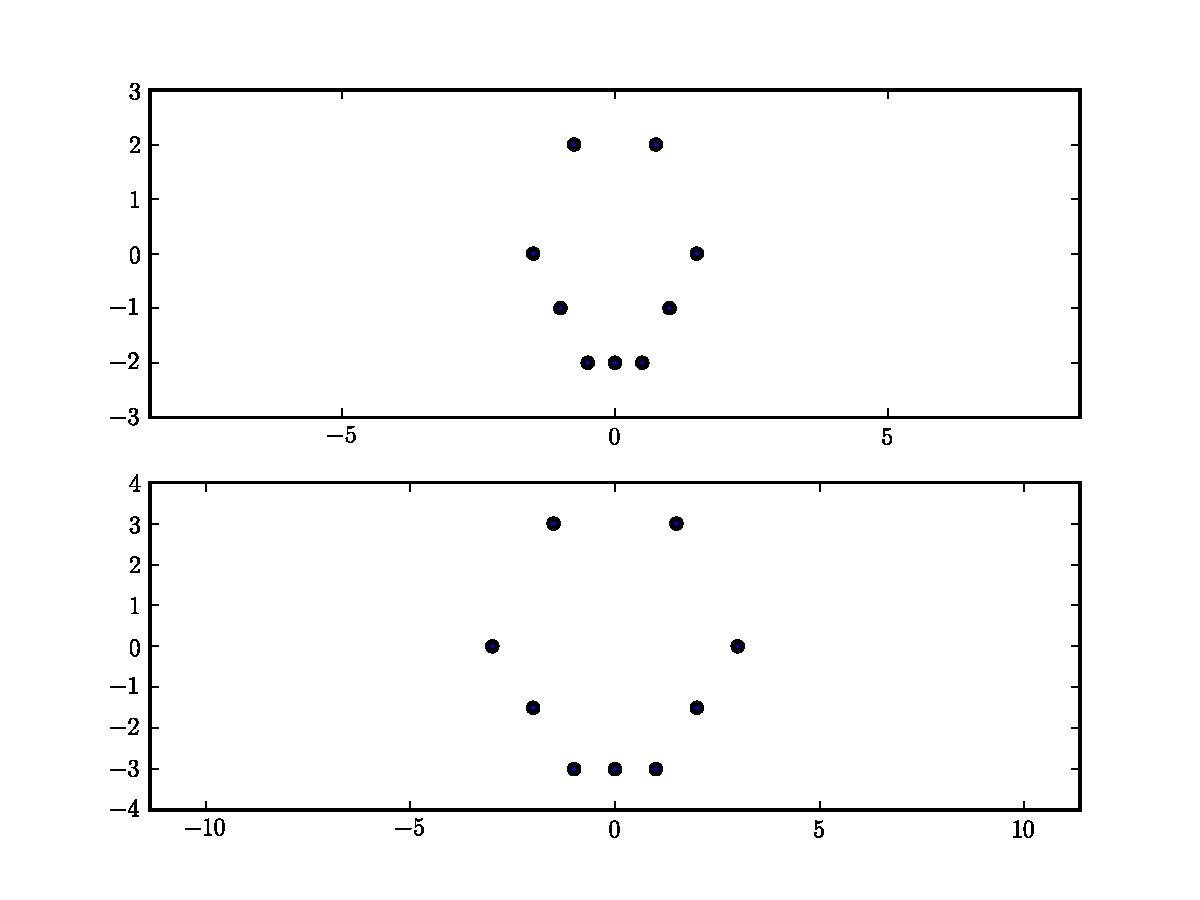
\includegraphics[width=\textwidth]{stretch.pdf}
\caption{
An example of a stretch, the top image is the original image and the bottom is the modified image.
The stretch was $2$ in the $x$ direction and $1.5$ in the $y$ direction.}
\end{figure}

\begin{problem}
Write a function that accepts an array of points and how much to stretch them in each direction.
Plot the transformed points.
This can be done with the following code:
\begin{lstlisting}
import numpy as np
# now construct an array 'pts' with
# x values along its first row and
# y values along its second row
from matplotlib import pyplot as plt
plt.scatter(pts[0], pts[1])
plt.show()
\end{lstlisting}
\end{problem}

\section*{Rotation}

To perform a rotation $\theta$ radians counterclockwise let
\[
A = \begin{pmatrix}
\cos(\theta) & -\sin(\theta) \\
\sin(\theta) & \cos(\theta) 
\end{pmatrix}
\]

\begin{figure}
\centering
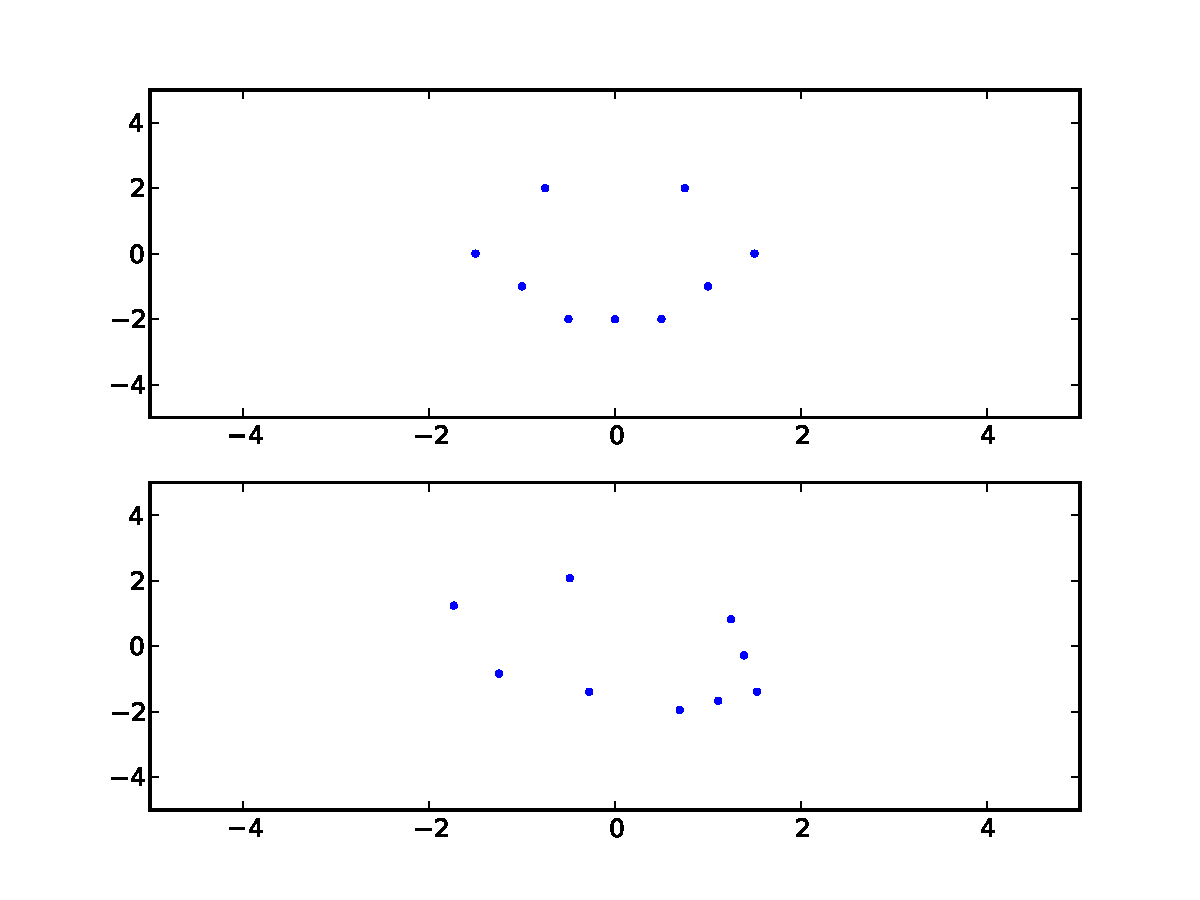
\includegraphics[width=\textwidth]{rotate.pdf}
\caption{An example of a rotation.
The top image is the original and the bottom is the rotated image.
The rotation angle is $\frac{3\pi}{16}$.}
\end{figure}

\begin{problem}
Write a function that will accept an array of points and how many radians to rotate them.
Have it return the rotated version of the points.
Plot the original points and their image under the transformation.
\end{problem}

\section*{Shift}

Shifts are not linear transformations, but they can be performed easily with array operations.
They are a part of a broader class of transformations called ``affine transformations."
These are transformations of the form $T: \mathbb{R}^n \to \mathbb{R}^n$, $T(x) = A x + b$ where $A$ is an $n\times n$ matrix and $b \in \mathbb{R}^n$.
Affine transformations include all compositions of stretches, rotations, and shifts.

Let $b$ be a vector that represents the desired shift.
In order to shift a set of points, you add to the row how much you would like it to shift it in that direction, so to shift the set of points up by 2, \li{b = np.array([0,2])}.
This particular shape for $b$ allows for proper array broadcasting.

\begin{figure}
\centering
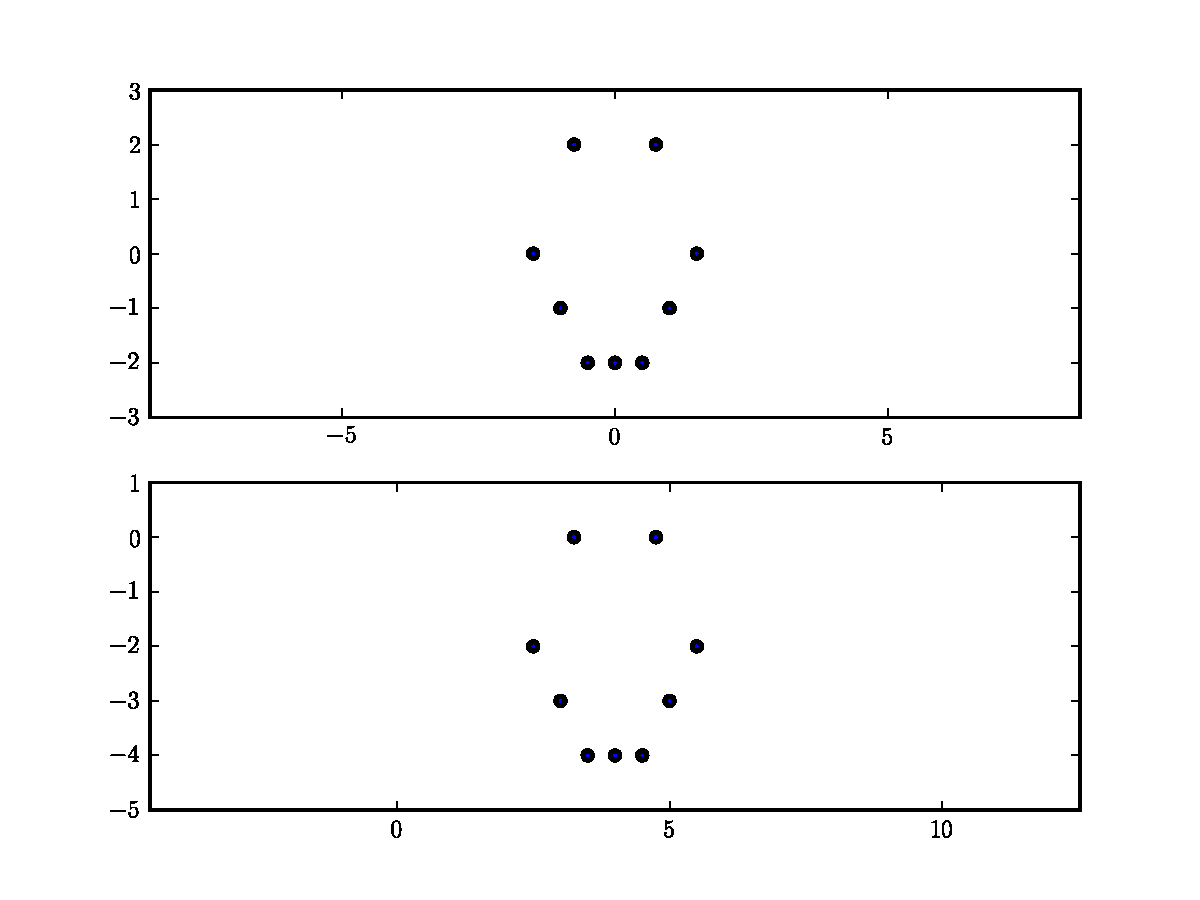
\includegraphics[width=\textwidth]{shift.pdf}
\caption{
An example of a shift.
The top image is the original and the bottom is the modified image.
The shift was $2$ in the $x$ direction and $1$ in the $y$ direction.}
\end{figure}

\begin{problem}
Write a function that takes an array of points and how much to shift them in each direction and returns the image of the points under the desired shift.
\end{problem}

\section*{Combination}
These transformations can be combined into single affine transformations through function composition.
For example, if you want to apply a stretch and then a rotation, you can represent the stretch as a matrix $S$ and the rotation as a matrix $R$ and represent the combined transformation as $R S$.
The image of $x$ under both transformations will be $R S x$.
An example like this is shown in Figure \ref{basis:combo}.


\begin{figure}
\centering
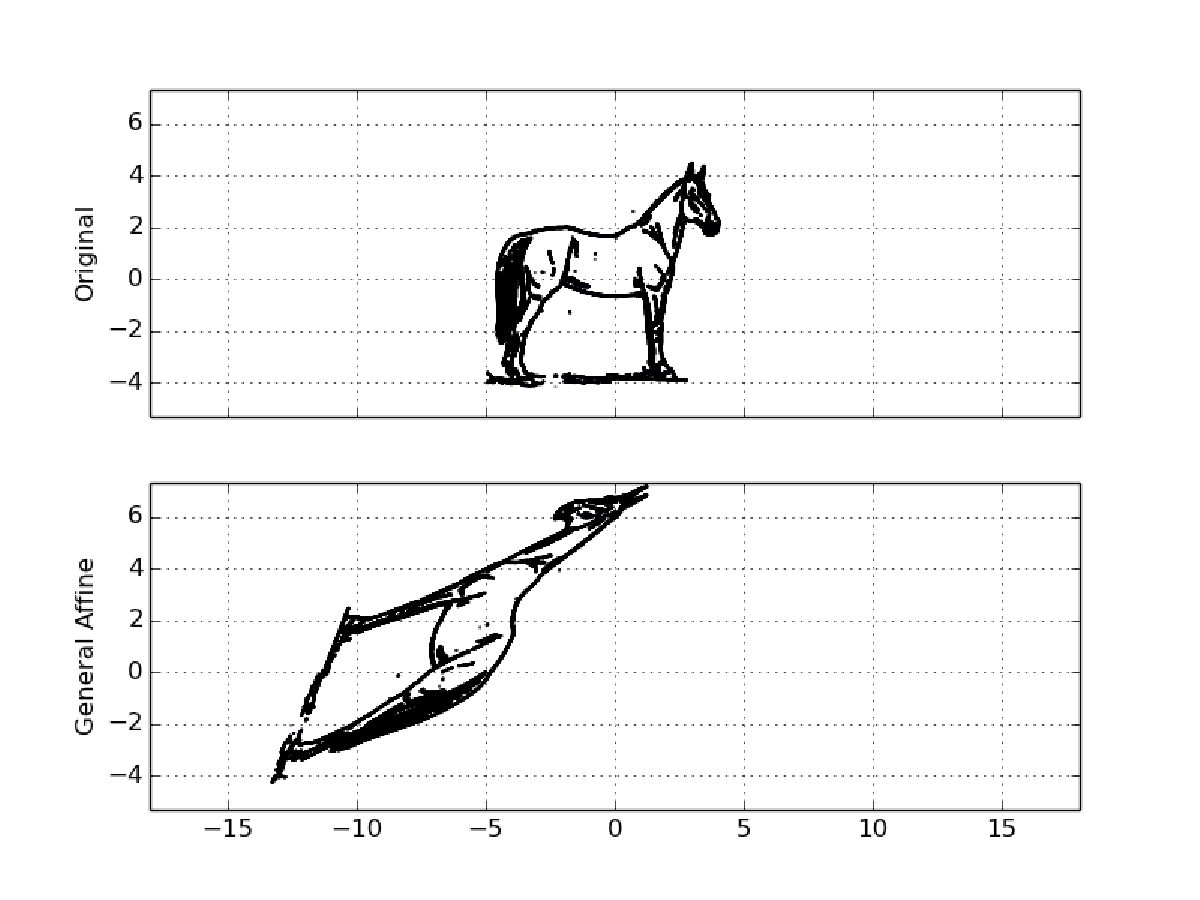
\includegraphics[width=\textwidth]{combo.pdf}
\caption{
A combination of linear transformations.
The stretch was $2$ in each direction.
The rotation angle was $\frac{3\pi}{4}$.
The shift was $1$ in the $x$ direction and $-2$ in the $y$ direction.}
\label{basis:combo}
\end{figure}

\begin{problem}
Write a function that rotates and shifts an array of points.
\end{problem}

\section*{Images}
An Image is a 3D array where the first two dimensions are the location and the 3rd dimension is the RGB content. To apply the above transformations one would need to moved the position of the RGB arrays to match where the new transformation would have them. Stretching is done by interpolation.

An Image can be represented as a 3d array where the indices along the first two dimensions represent pixel location within the image and the 3rd dimension is the RGB content.
To apply the above transformations one would need to move the position of the RGB arrays to match where the new transformation would have them.

\begin{figure}
\centering

\includegraphics[scale=2.0]{dream.png}
\caption{The original image}
\label{basis:image}
\end{figure}

\begin{figure}
\centering
\includegraphics[width=\textwidth]{rotateimg.pdf}
\caption{The image in Figure \ref{basis:image} rotated $\frac{\pi}{4}$ radians counterclockwise.}
\end{figure}

TODO: clarify how to actually do this and plot it.

\begin{problem}
Write a function that rotates an image a given number of radians.
HINTS: Make an array of ones that is $1.5$ times greater than the maximum height and width of the original image.
Change the $x$ and $y$ coordinates in the original image so that center is $(0,0)$, then rotate the image.
You might need to use some for-loops.
Make your test cases relatively small images.
\end{problem}


